\documentclass{article}

\usepackage{tikz}
\usepackage{tikz-qtree}

\newcommand\leaf[3]{\makebox[5em][l]{#1}\texttt{#2\ldots#3\ldots}}

\newcommand\April     {\leaf{April     }{ 41 70 72 }{ 0100 0001 0111 0000 0111 0010 }}
\newcommand\August    {\leaf{August    }{ 41 75 67 }{ 0100 0001 0111 0101 0110 0111 }}
\newcommand\December  {\leaf{December  }{ 44 65 63 }{ 0100 0100 0110 0101 0110 0011 }}
\newcommand\February  {\leaf{February  }{ 46 65 62 }{ 0100 0110 0110 0101 0110 0010 }}
\newcommand\January   {\leaf{January   }{ 4a 61 6e }{ 0100 1010 0110 0001 0110 1110 }}
\newcommand\July      {\leaf{July      }{ 4a 75 6c }{ 0100 1010 0111 0101 0110 1100 }}
\newcommand\June      {\leaf{June      }{ 4a 75 6e }{ 0100 1010 0111 0101 0110 1110 }}
\newcommand\March     {\leaf{March     }{ 4d 61 72 }{ 0100 1101 0110 0001 0111 0010 }}
\newcommand\May       {\leaf{May       }{ 4d 61 79 }{ 0100 1101 0110 0001 0111 1001 }}
\newcommand\November  {\leaf{November  }{ 4e 6f 76 }{ 0100 1110 0110 1111 0111 0110 }}
\newcommand\October   {\leaf{October   }{ 4f 63 74 }{ 0100 1111 0110 0011 0111 0100 }}
\newcommand\September {\leaf{September }{ 53 65 70 }{ 0101 0011 0110 0101 0111 0000 }}

\begin{document}

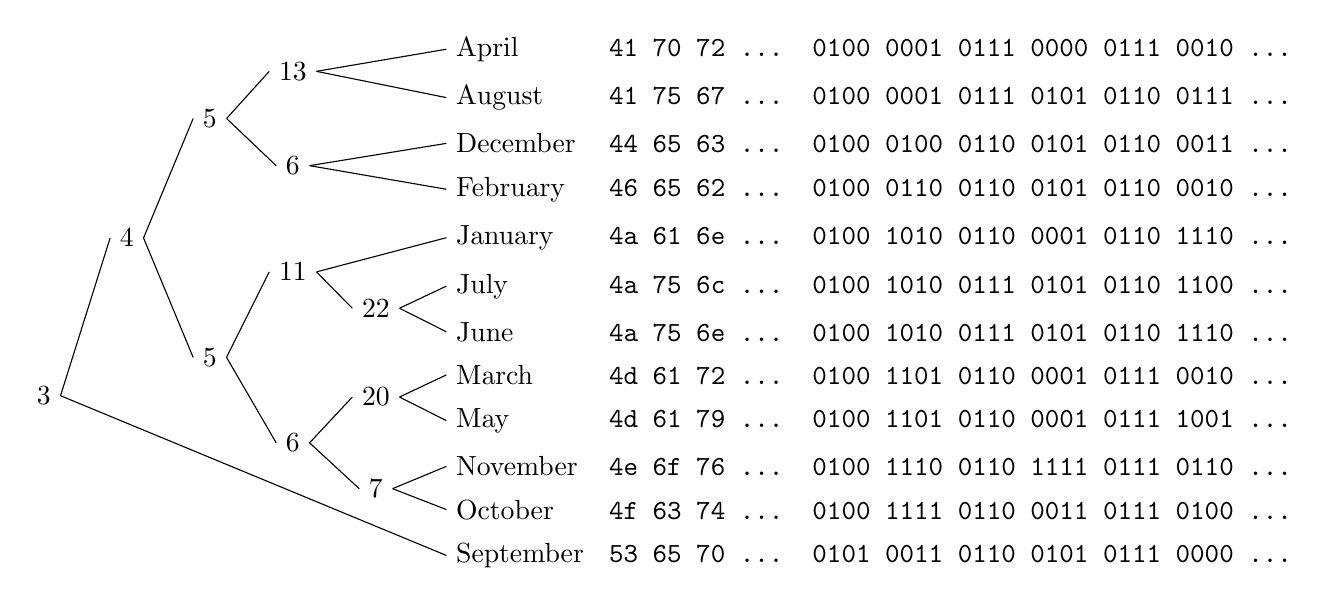
\begin{tikzpicture}

\tikzset{grow'=right,level distance=3em}
\tikzset{frontier/.style={distance from root=30em}}

\Tree [.3 [.4 [.5              [.13           {\April}
                                              {\August} ]
                  [.6                         {\December}
                                              {\February} ] ]
              [.5         [.11                {\January}
                                         [.22 {\July}
                                              {\June} ] ]
                  [.6               [.20      {\March}
                                              {\May} ]
                      [.7                     {\November}
                                              {\October} ] ] ] ]
                                              {\September} ]

\end{tikzpicture}

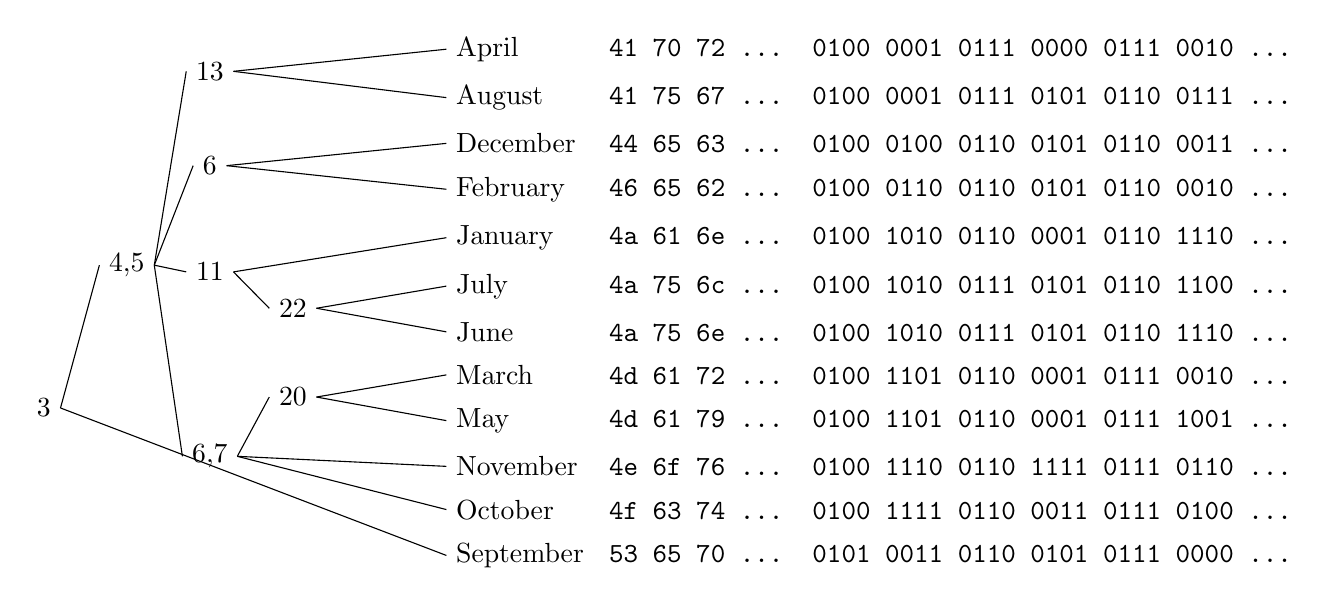
\begin{tikzpicture}

\tikzset{grow'=right,level distance=3em}
\tikzset{frontier/.style={distance from root=30em}}

\Tree [.3 [.4,5            [.13           {\April}
                                          {\August} ]
                [.6                       {\December}
                                          {\February} ]
                      [.11                {\January}
                                     [.22 {\July}
                                          {\June} ] ]
                [.6,7           [.20      {\March}
                                          {\May} ]
                                          {\November}
                                          {\October} ] ]
                                          {\September} ]

\end{tikzpicture}

\begin{tikzpicture}
[row 2/.style={font=\scriptsize}
,row 3/.style={font=\scriptsize}
,every matrix/.style={draw,nodes={text width=1em,align=center}}
]

\matrix(13) at      (5,9)  { \node{13}; \\ \node(130){0}; \\ \node(131){1}; \\ };
\matrix(5a) at   (2,8)     { \node{5};  \\ \node(5a0){0}; \\ \node(5a1){1}; \\ };
\matrix(6a) at    (3,7)    { \node{6};  \\ \node(6a0){0}; \\ \node(6a1){1}; \\ };
\matrix(4)  at  (1,6)      { \node{4};  \\ \node(4x0){0}; \\ \node(4x1){1}; \\ };
\matrix(11) at      (5,5)  { \node{11}; \\ \node(110){0}; \\ \node(111){1}; \\ };
\matrix(22) at       (6,4) { \node{22}; \\ \node(220){0}; \\ \node(221){1}; \\ };
\matrix(5b) at   (2,3)     { \node{5};  \\ \node(5b0){0}; \\ \node(5b1){1}; \\ };
\matrix(20) at       (6,2) { \node{20}; \\ \node(200){0}; \\ \node(201){1}; \\ };
\matrix(6b) at    (3,1)    { \node{6};  \\ \node(6b0){0}; \\ \node(6b1){1}; \\ };
\matrix(7)  at     (4,0)   { \node{7};  \\ \node(7x0){0}; \\ \node(7x1){1}; \\ };
\matrix(3)  at (0,5)       { \node{3};  \\ \node(3x0){0}; \\ \node(3x1){1}; \\ };

\draw [->] (node cs:name=3,angle=0) .. controls +(1,0) and +(-1,0) .. (node cs:name=4,angle=140);
\draw [->] (node cs:name=4,angle=0) -> (5a.south);
\draw [->] (node cs:name=4,angle=-30) -> (5b.north);

\end{tikzpicture}

\end{document}
